\documentclass[dvipdfmx]{jarticle}
\usepackage{tikz}
\usetikzlibrary{calc,shapes}
\pagestyle{empty}
\begin{document}
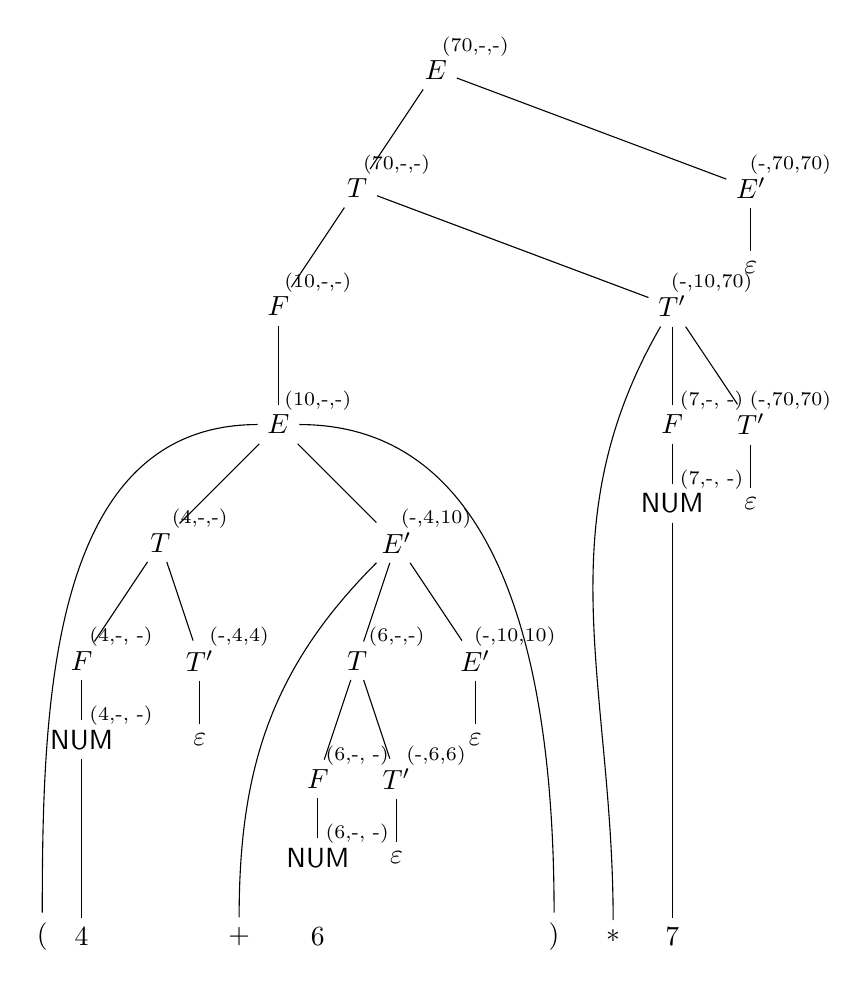
\begin{tikzpicture}
\node (R) at (0,0) {$E$};
\node (T1) at ($(R)+(-1,-1.5)$) {$T$};
\node (E'1) at ($(R)+(4,-1.5)$) {$E'$};
\node (e5) at ($(E'1)+(0,-1)$) {$\varepsilon$};
\node (F1) at ($(T1)+(-1,-1.5)$) {$F$};
\node (T'1) at ($(T1)+(4,-1.5)$) {$T'$};
\node (E1) at ($(F1)+(0,-1.5)$) {$E$};
\node (T2) at ($(E1)+(-1.5,-1.5)$) {$T$};
\node (E'2) at ($(E1)+(1.5,-1.5)$) {$E'$};
\node (F2) at ($(T2)+(-1,-1.5)$) {$F$};
\node (T'2) at ($(T2)+(0.5,-1.5)$) {$T'$};
\node (N1) at ($(F2)+(0,-1)$) {$\mathsf{NUM}$};
\node (e1) at ($(T'2)+(0,-1)$) {$\varepsilon$};
\node (T3) at ($(E'2)+(-0.5,-1.5)$) {$T$};
\node (E'3) at ($(E'2)+(1,-1.5)$) {$E'$};
\node (e3) at ($(E'3)+(0,-1)$) {$\varepsilon$};
\node (F3) at ($(T3)+(-0.5,-1.5)$) {$F$};
\node (T'3) at ($(T3)+(0.5,-1.5)$) {$T'$};
\node (N2) at ($(F3)+(0,-1)$) {$\mathsf{NUM}$};
\node (e2) at ($(T'3)+(0,-1)$) {$\varepsilon$};
\node (F4) at ($(T'1)+(0,-1.5)$) {$F$};
\node (T'4) at ($(T'1)+(1,-1.5)$) {$T'$};
\node (N3) at ($(F4)+(0,-1)$) {$\mathsf{NUM}$};
\node (e4) at ($(T'4)+(0,-1)$) {$\varepsilon$};
\node (w1) at ($(N1)+(0,-2.5)$) {$4$};
\node (w0) at ($(w1)+(-0.5,0)$) {$($};
\node (w2) at ($(w1)+(2,0)$) {$+$};
\node (w3) at ($(N2)+(0,-1)$) {$6$};
\node (w4) at ($(w3)+(3,0)$) {$)$};
\node (w6) at ($(N3)+(0,-5.5)$) {$7$};
\node (w5) at ($(w4)+(0.75,0)$) {$\ast$};
\path[-] (R) edge (T1) (R) edge (E'1);
\path[-] (T1) edge (F1) (T1) edge (T'1);
\path[-] (E'1) edge (e5);
\path[-] (F1) edge (E1);
\path[-] (E1) edge (T2) (E1) edge (E'2);
\path[-] (T2) edge (F2) (T2) edge (T'2);
\path[-] (F2) edge (N1) (T'2) edge (e1);
\path[-] (E'2) edge (T3) (E'2) edge (E'3);
\path[-] (T3) edge (F3) (T3) edge (T'3);
\path[-] (F3) edge (N2) (T'3) edge (e2);
\path[-] (E'3) edge (e3);
\path[-] (T'1) edge (F4) (T'1) edge (T'4);
\path[-] (F4) edge (N3) (T'4) edge (e4);
\path[-] (N1) edge (w1);
\path[-] (N3) edge (w6);
\path[-] (E1) [out=180,in=90] edge (w0);
\path[-] (E1) [out=0,in=90] edge (w4);
\path[-] (E'2) [out=225,in=90] edge (w2);
\path[-] (T'1) [out=240,in=90] edge (w5);

\node at ($(N1)+(0.5,0.3)$) {\scriptsize (4,-, -)};
\node at ($(N2)+(0.5,0.3)$) {\scriptsize (6,-, -)};
\node at ($(N3)+(0.5,0.3)$) {\scriptsize (7,-, -)};
\node at ($(F2)+(0.5,0.3)$) {\scriptsize (4,-, -)};
\node at ($(F3)+(0.5,0.3)$) {\scriptsize (6,-, -)};
\node at ($(F4)+(0.5,0.3)$) {\scriptsize (7,-, -)};
\node at ($(T'2)+(0.5,0.3)$) {\scriptsize (-,4,4)};
\node at ($(T2)+(0.5,0.3)$) {\scriptsize (4,-,-)};
\node at ($(T'3)+(0.5,0.3)$) {\scriptsize (-,6,6)};
\node at ($(T3)+(0.5,0.3)$) {\scriptsize (6,-,-)};
\node at ($(E'3)+(0.5,0.3)$) {\scriptsize (-,10,10)};
\node at ($(E'2)+(0.5,0.3)$) {\scriptsize (-,4,10)};
\node at ($(E1)+(0.5,0.3)$) {\scriptsize (10,-,-)};
\node at ($(T'4)+(0.5,0.3)$) {\scriptsize (-,70,70)};
\node at ($(T'1)+(0.5,0.3)$) {\scriptsize (-,10,70)};
\node at ($(F1)+(0.5,0.3)$) {\scriptsize (10,-,-)};
\node at ($(T1)+(0.5,0.3)$) {\scriptsize (70,-,-)};
\node at ($(E'1)+(0.5,0.3)$) {\scriptsize (-,70,70)};
\node at ($(R)+(0.5,0.3)$) {\scriptsize (70,-,-)};
\end{tikzpicture}
\end{document}